
\documentclass[tikz, border=1mm]{standalone}

\usepackage{amsmath}

\usetikzlibrary{calc,angles,quotes,intersections,shapes.geometric}

\usepackage{tkz-euclide}

\begin{document}
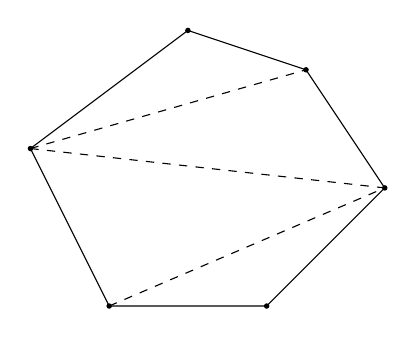
\begin{tikzpicture}[scale=0.5]

	% ---- coordinates

	\coordinate (P1) at (0,0);
	\coordinate (P2) at (-2,4);
	\coordinate (P3) at (2,7);
	\coordinate (P4) at (5,6);
	\coordinate (P5) at (7,3);
	\coordinate (P6) at (4,0);

	% ---- polygon

	\draw (P1) \foreach \i in {2,...,6} { -- (P\i) } -- cycle;

	% ---- triangles

	\draw[dashed] (P2) -- (P4);
	\draw[dashed] (P2) -- (P5);
	\draw[dashed] (P1) -- (P5);

	% ---- thick vertices

	\foreach \i in {1,...,6} { \fill (P\i) circle (0.7mm); }

\end{tikzpicture}
\end{document}
